\begin{lemma}%Lemma 6.1 Munkres
	Let $L$ be the complex depicted in figure \ref{rectangle-tri}, whose underlying space is a rectangle. Let $\mathrm{Bd} L$ denote the complex whose space is the boundary of the rectangle. Orient each 2-simplex $\sigma_i$ of $L$ counterclockwise. Orient the 1-simplices arbitrarily. Then:
	\begin{enumerate}
		\item Every 1-cycle of $L$ is homologous to a 1-cycle carried by $\mathrm{Bd} L$.
		\item If $d$ is a 2-chain of $L$ and if $\partial d$ is carried by $\mathrm{Bd}L$, then $d$ is a multiple of the chain $\sum \sigma_i$.
	\end{enumerate} 
\end{lemma}
% A chain c is carried by a subcomplex $L$ of $K$ if $c$ has value 0 on every simplex that is not in $L$. We say two chais are homologous if they only differ by a boundary.


\begin{figure}\begin{center}
	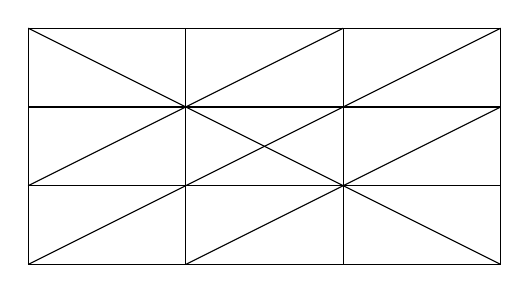
\begin{tikzpicture}[yscale=0.5]
	\draw (0,0)--(6,0)--(6,6)--(0,6)--cycle;
	\draw (2,0)--(2,6);
	\draw (4,0)--(4,6);
	\draw (0,2)--(6,2);
	\draw (0,4)--(6,4);
	\draw (0,6)--(6,0);
	\draw (0,2)--(4,6);
	\draw (0,0)--(6,6);
	\draw (2,0)--(6,4);
	\end{tikzpicture}	
	\caption{Complex whose underlying space is a rectangle.\label{rectangle-tri}}

\end{center}
\end{figure}


\begin{proof}
	We will prove the second statement fist. If $\sigma_i$ and $\sigma_j$ have an edge $e$ in common, then $\partial d$ must have value 0 on $e$. It follows that $d$ must have the same value $\sigma_i$ as it does in $\sigma_j$. Continuing this process, we see that $d$ has the same value on every oriented 2-simplex $\sigma_i$.
	
	For the second part, let $c$ be be a 1-chain of $L$. We will \glqq push it off \grqq{} the 1-simplices in the following way:
	
	We concentrate on the center at first. There we notice the structure as depicted in figure \ref{zoom-in}.
	
	\begin{figure}
		\begin{center}
			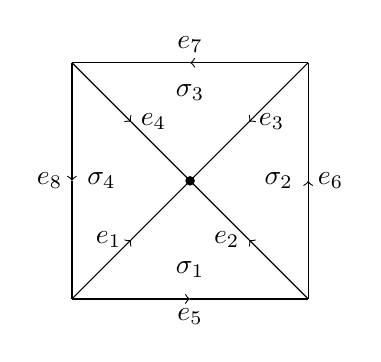
\begin{tikzpicture}[scale=1.5]
				\draw[->] (0,0)->(1,0) node[below]{$e_5$};
				\draw (1,0)--(2,0);
				\draw[->] (2,0)->(2,1) node[right]{$e_6$};
				\draw (2,1)--(2,2);
				\draw[->] (2,2)->(1,2) node[above]{$e_7$};
				\draw (1,2)--(0,2);
				\draw[->] (0,2)->(0,1) node[left]{$e_8$};
				\draw (0,1)--(0,0);
				\draw[->] (0,0)--(0.5,0.5) node[left]{$e_1$};
				\draw (0.5,0.5)--(1.5,1.5);
				\draw (1.5,0.5)--(0.5,1.5);
				\draw[->](2,2)--(1.5,1.5) node[right]{$e_3$};
				\draw[->](2,0)--(1.5,0.5) node[left]{$e_2$};
				\draw[->](0,2)--(0.5,1.5) node[right]{$e_4$};
				\filldraw (1,1) circle (1pt);
				\draw (1,0.25) node{$\sigma_1$};
				\draw (1,1.75) node{$\sigma_3$};
				\draw (0.25,1) node{$\sigma_4$};
				\draw (1.75,1) node{$\sigma_2$};
			\end{tikzpicture}
			\caption{Structure of center. 2-simplices are oriented counterclockwise\label{zoom-in}}
		\end{center}
	\end{figure}

Let $c$ denote a 1-chain with value $a$ on $e_1$. Then $c$ is clearly homologous to the chain $c_1=c+\partial(a\sigma_1)$. The resulting 1-chain $c_1$ vanishes on $e_1$. We have \glqq pushed it off\grqq{} $e_1$. We can apply this multiple times for other edges until we arrive at a chain $c_2$ which is carried by the subcomplex depicted in figure \ref{skelleton}
\begin{figure}
	\begin{center}
		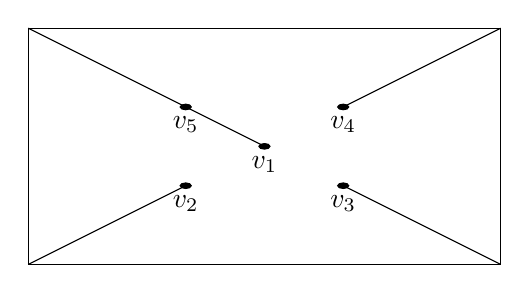
\begin{tikzpicture}[yscale=0.5]
		\draw (0,0)--(6,0)--(6,6)--(0,6)--cycle;
		\draw (0,6)--(3,3);
		\draw (0,0)--(2,2);
		\draw (6,0)--(4,2);
		\draw (6,6)--(4,4);
		\filldraw (2,2)circle(2pt) node[below]{$v_2$};
		\filldraw (3,3)circle(2pt) node[below]{$v_1$};
		\filldraw (2,4)circle(2pt) node[below]{$v_5$};
		\filldraw (4,4)circle(2pt) node[below]{$v_4$};
		\filldraw (4,2)circle(2pt) node[below]{$v_3$};
		\end{tikzpicture}
		\caption{Subcomplex that carries $c_2$.\label{skelleton}}	
	\end{center}
\end{figure} 

Since our original $c$ is a cycle, $c_2$ must be carried by $\mathrm{Bd} L$, because otherwise $\partial c_2$ 
%TODO Check boundary here? In Munkres no boundary.
would have non-zero coefficients on one or more of the vertices $v_1, \dots,v_5$.
\end{proof}

\begin{theorem}
	Let $T$ denote the complex represented by the labeled rectangle $L$ of Figure \ref{torus-tri}. Its underlying space is the torus. Then:
	\[H_1(T)\isom \Z\oplus\Z \qandq H_2(T)\isom \Z.\]
	Orient each 2-simplex of $L$ counterclockwise; use the induced orientation of the 2-simplices of T; Let $\gamma$ denote their sum. Let 
	\begin{align*}
	w_1=&[a,b]+[b,c]+[c,a],\\
	z_1=&[a,d]+[d,e]+[e,a].
	\end{align*}
	Then $\gamma$ generates $H_2(T)$ and $w_1$ and $z_1$ represent a basis for $H_1(T)$.
\end{theorem}

\begin{figure}\begin{center}
		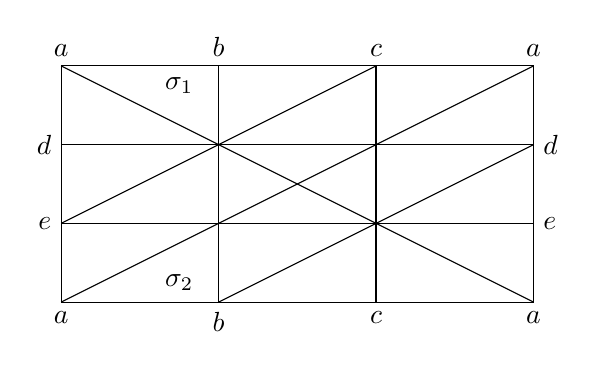
\begin{tikzpicture}[yscale=0.5]
		\draw (0,0) node[below]{$a$}--(6,0)node[below]{$a$}--(6,6)node[above]{$a$}--(0,6)node[above]{$a$}--cycle;
		\draw (2,0)node[below]{$b$}--(2,6)node[above]{$b$};
		\draw (4,0)node[below]{$c$}--(4,6)node[above]{$c$};
		\draw (0,2)node[left]{$e$}--(6,2)node[right]{$e$};
		\draw (0,4)node[left]{$d$}--(6,4)node[right]{$d$};
		\draw (0,6)--(6,0);
		\draw (0,2)--(4,6);
		\draw (0,0)--(6,6);
		\draw (2,0)--(6,4);
		\draw (1.5,5.5)node{$\sigma_1$};
		\draw (1.5,0.5) node{$\sigma_2$};
		\end{tikzpicture}	
		\caption{Labeled Complex whose underlying space is a torus.\label{torus-tri}}
		
	\end{center}
\end{figure}
\begin{proof}
	Let $g: |L|\to |T|$ be the pasting (gluing) map; let $A=g(|\mathrm{Bd} L)$. Then $A$ is homeomorphic to\footnote{The wedge sum is the disjoint union where two points are identified.} $\Sp^1\wedge \Sp^1$ as depicted in figure \ref{wege-of-s1}. Orient the 1-simplices of $T$ arbitrarily. Since $g$ only identifies simplices in $\mathrm{Bd} L$, we find the same statements as above with identical arguments.
	\begin{enumerate}
		\item \label{gen-1}Every 1-cycle of $T$ is homologous to a 1-cycle carried by $A$.
		\item \label{gen-2}If $d$ is a 2-chain of $T$ and if $\partial d$ is carried by $A$, then $d$ is a multiple of $\gamma$.
	\end{enumerate}
	Additionally, we find here
	\begin{enumerate}\setcounter{enumi}{2}
		\item \label{torus-1} If $c$ is a 1-cycle of $T$ carried by $A$, then $c$ is of the form $nw_1+mz_1$.
		\item \label{torus-2}$\partial \gamma=0$.
	\end{enumerate} 
	\begin{figure}
		\begin{center}
			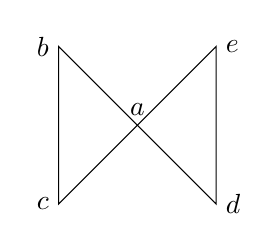
\begin{tikzpicture}
				\draw (-1,-1) node[left]{$c$}--(0,0) node[above]{$a$}--(-1,1) node[left]{$b$}--cycle;
				\draw (0,0)--(1,-1) node[right]{$d$}--(1,1)node[right]{$e$}--cycle;
			\end{tikzpicture}
			\caption{$A$ is homeomorphic to $\Sp^1\wedge \Sp^1$\label{wege-of-s1}}
		\end{center}
	\end{figure}

The statement in item \ref{torus-1} is clear by looking at figure \ref{wege-of-s1}. For item \ref{torus} we need to see the following: 
It is clear that $\partial\gamma$ vanishes on any 1-simplex not contained in $A$. By direct computation one can see that $\partial\gamma$ also vanishes on all 1-simplices in $A$. The 1-simplex $[a,b]$ appears as a face of $\sigma_1$ and $\sigma_2$ and no other simplices. If we evaluate $\partial\sigma_1$ the elementary chain $[a,b]$ is assigned the value $-1$ and evaluating $\partial\sigma_2$ gives $+1$ for $[a,b]$.

Combining all of the results above yields the homology groups of $T$:
Every 1-cycle of $T$ is homologous to a 1-cycle of the form $c=nw_1+mz_1$ by \ref{gen-1} and \ref{torus-1}. Such a cycle bounds only if it is trivial: If $c=\partial d$ for some $d$, then by virtue of \ref{gen-2} $d=p\gamma$ for some integer $p$. By \ref{torus-2} we know that $\partial\gamma=0$, so $c=0$. Therefore,
\[H_1(T)\isom\Z\oplus\Z; \]
with base elements $w_1$ and $z_1$.

For dimension 2,we find that any 2-cycle $d$ of $T$ must be of the form $p\gamma$ for some $p$ by virtue of \ref{gen-2}. Such a 2-chain is always a cycle, by \ref{torus-2}, and there are no 3-chains whose boundary they could be, hence
\[
H_2(T)\isom \Z
\]
with generator $\gamma$.
\end{proof}




\begin{theorem}
	let $S$ denote the complex represented by the labeled rectangle of figure \ref{klein-tri}; its underlying space is the Klein bottle. Then 
	\[H_1(S)\isom\Z\oplus\Z_2\qandq H_2(S)=0.\]
	The torsion element of $H_1(S)$ is represented by the chain $z_1$, and a generator for the group $H_1(S)$ modulo torsion is represented by $w_1$, where
	\begin{align*}
		w_1&=[a,b]+[b,c]+[c,a]\\
		z_1&=[a,d]+[d,e]+[e,a].
	\end{align*}
\end{theorem}
\begin{figure}\begin{center}
		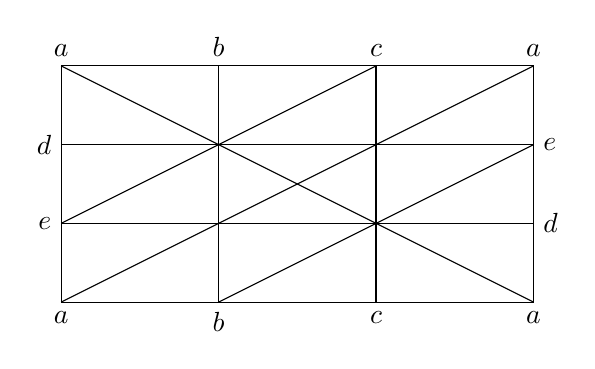
\begin{tikzpicture}[yscale=0.5]
		\draw (0,0) node[below]{$a$}--(6,0)node[below]{$a$}--(6,6)node[above]{$a$}--(0,6)node[above]{$a$}--cycle;
		\draw (2,0)node[below]{$b$}--(2,6)node[above]{$b$};
		\draw (4,0)node[below]{$c$}--(4,6)node[above]{$c$};
		\draw (0,2)node[left]{$e$}--(6,2)node[right]{$d$};
		\draw (0,4)node[left]{$d$}--(6,4)node[right]{$e$};
		\draw (0,6)--(6,0);
		\draw (0,2)--(4,6);
		\draw (0,0)--(6,6);
		\draw (2,0)--(6,4);
		\end{tikzpicture}	
		\caption{Labeled Complex whose underlying space is the Klein bottle.\label{klein-tri}}
		
	\end{center}
\end{figure}
\begin{proof}
	Let $g$ and $A$ be as before with the obvious changes. Again, $A$ is homeomorphic to $\Sp^1\wedge \Sp^1$. Orient all 2-simplices of $S$ as before and let $\gamma$ be their sum. Orient the 1-simplices arbitrarily. Once more, Statements \ref{gen-1} and \ref{gen-2} from the previous proof hold for the same reason as before. Since $A$ is the wedge sum of two circles again, \ref{torus-1} holds again. However, condition \ref{torus-2} needs to be modified:
	\begin{enumerate}
		\setcounter{enumi}{3}
		\item $\partial \gamma=2z_1$\label{klein-2}.
	\end{enumerate}
	This result can be obtained via a direct calculation similar from what we did before.
	
	By \ref{gen-1} and \ref{torus-1} we know that every 1-cycle of $S$ is homologous to a cycle of the form $c=nw_1+mz_1$. If $c$ is a boundary for some $d$, then \ref{gen-2} implies $d=p\gamma$. Thus, $\partial d=2pz_1$. Therefore $nw_1+mz_1$ bounds if and only if $m$ is even and $n$ is zero. Thus,
	\[H_1(S)\isom\Z\oplus\Z_2\]
	The cycle $z_1$ represents the torsion element, and $w_1$ represents a generator of the infinite cyclic group $H_1(S)/T_1(S)$.
	
	For the second homology group, note that any 2-cycle $d$ of $S$ must be of the form $p\gamma$ by \ref{gen-2}. \ref{klein-2} implies that $p\gamma$ is not a cycle, hence
	\[
	H_2(S)=0.
	\]
\end{proof}